% Created 2019-01-16 Wed 21:39
% Intended LaTeX compiler: pdflatex
\documentclass[12pt, letterpaper]{paper}
\usepackage[utf8]{inputenc}
\usepackage[T1]{fontenc}
\usepackage{graphicx}
\usepackage{grffile}
\usepackage{longtable}
\usepackage{wrapfig}
\usepackage{rotating}
\usepackage[normalem]{ulem}
\usepackage{amsmath}
\usepackage{textcomp}
\usepackage{amssymb}
\usepackage{capt-of}
\usepackage{hyperref}
\usepackage{Schwieg}
\usepackage{natbib}
\usepackage{tikz}
\usepackage{bm}
\usepackage{minted}
\usepackage[margin=1in]{geometry}
\usepackage{fontspec}
\setmonofont{DejaVu Sans Mono}[Scale=MatchLowercase]
\author{Timothy Schwieg}
\date{\today}
\title{Structural Estimation Pset 2}
\hypersetup{
 pdfauthor={Timothy Schwieg},
 pdftitle={Structural Estimation Pset 2},
 pdfkeywords={},
 pdfsubject={},
 pdfcreator={Emacs 26.1 (Org mode 9.1.9)}, 
 pdflang={English}}
\begin{document}

\maketitle

\section{Question One}
\label{sec:org2ded0c1}
\subsection{a}
\label{sec:org83aad7c}
\begin{minted}[frame=lines,fontsize=\scriptsize,xleftmargin=\parindent,linenos,mathescape,breaklines=true,stripnl=true,firstnumber=last]{julia}
#healthClaims = CSV.read( "clms.txt", header=[:A] )
healthClaims = DataFrame(load("clms.csv", header_exists=false, colnames=["A"]))
#describe( healthClaims )
#println( "Standard Deviation: ", std(healthClaims[:A]))

results = [["mean", "min", "median", "max", "StdDev"] cln.([mean(healthClaims[:A]), minimum(healthClaims[:A]), median(healthClaims[:A]), maximum(healthClaims[:A]), std(healthClaims[:A])] )]
\end{minted}

\begin{center}
\begin{tabular}{lr}
mean & 720.28\\
min & 0.01\\
median & 172.21\\
max & 2.2797 \texttimes{} 10\(^{\text{05}}\)\\
StdDev & 3972.9\\
\end{tabular}
\end{center}

\begin{minted}[frame=lines,fontsize=\scriptsize,xleftmargin=\parindent,linenos,mathescape,breaklines=true,stripnl=true,firstnumber=last]{julia}
histogram( healthClaims[:A], bins=1000, normalize = true, label="Health Claims")
savefig("histOne.png")
\end{minted}

\begin{center}
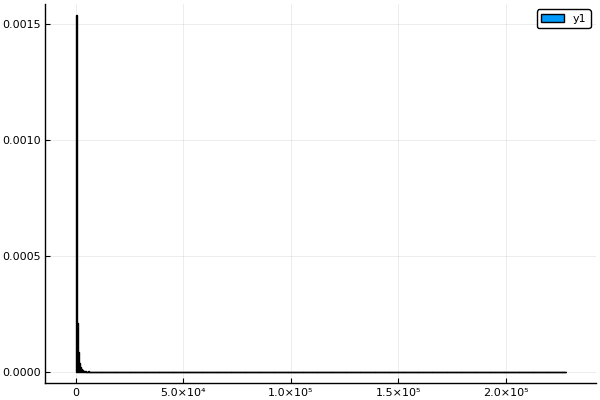
\includegraphics[width=.9\linewidth]{histOne.png}
\end{center}

\begin{minted}[frame=lines,fontsize=\scriptsize,xleftmargin=\parindent,linenos,mathescape,breaklines=true,stripnl=true,firstnumber=last]{julia}
  #We force all bins to have length 8, and allow for 100 of them.
histogram( healthClaims[:A], bins=0:8:800, normalize=true, xlims=(0,800),label="Health Claims \$\\leq 800\$")
savefig("histTwo.png")
\end{minted}

\begin{center}
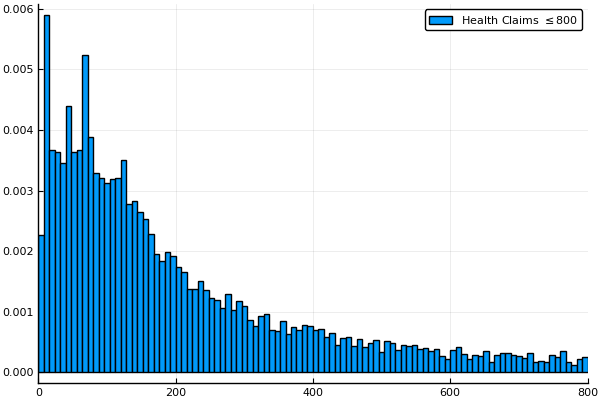
\includegraphics[width=.9\linewidth]{histTwo.png}
\end{center}



\subsection{b}
\label{sec:org1889832}
\begin{minted}[frame=lines,fontsize=\scriptsize,xleftmargin=\parindent,linenos,mathescape,breaklines=true,stripnl=true,firstnumber=last]{julia}
function GammaLogLikelihood( x::Vector{Float64}, α::Float64, β::Float64)
    #Yes I know I could get this using Distributions.jl which could
    #even do the MLE estimate But thats pretty much cheating, and
    #gamma is in the exponential family so using Newton's method will
    #cause no issues.

    #Pdf is: $\frac{ 1 }{\Gamma(\alpha) \beta^{\alpha}} x^{\alpha - 1} \exp\left( - \frac{x}{\beta} \right)$
    #Log-likelihood is: $- \alpha \log ( \beta) - \log( \Gamma (\alpha)) + (\alpha - 1) \log x - \frac{x}{\beta}$

    return -α*log( β) - lgamma(α) + (α - 1)*mean(log.(x)) - mean(x) / β
end

function GammaGradient( x::Vector{Float64}, α::Float64, β::Float64)
    delA = -log(β) - digamma(α) + mean(log.(x))
    #delB = mean(x) / β - α
    delB = mean(x) / β^2 - α / β
    return [delA,delB]
end

function GammaHessian( x::Vector{Float64}, α::Float64, β::Float64)
    delAA = -trigamma(α)
    delAB = -1 / β
    delBB =( α / (β*β)) - ((2* mean(x)) / (β*β*β))
    return [delAA delAB; delAB delBB]
end

function GammaPDF( α::Float64, β::Float64, x::Float64)
    return  (1 / (gamma(α)*β^α))*x^(α-1)*exp( -x/β)
end

function EstimateGammaParameters( data::Vector{Float64}, guess::Vector{Float64}, gradientFun, hessianFun)

    θ = guess
    tol = 1e-10
    maxLoops = 100

    grad = gradientFun( data, θ... )
    hess = hessianFun( data, θ... )

    loopCounter = 0
    while( loopCounter < maxLoops && norm(grad) >= tol)
        θ = θ - hess \ grad
        grad = gradientFun( data, θ... )
        hess = hessianFun( data, θ... )

        loopCounter += 1
        # println( norm(grad))
        # println( θ)
        # println( " ")
    end
    #println( loopCounter)
    return θ
end
healthCosts = convert(  Vector{Float64}, healthClaims[:A] )

β₀ =  var(healthCosts) / mean(healthCosts)
α₀ = mean(healthCosts) / β₀

(Gamma_̂α, Gamma_̂β) = EstimateGammaParameters( healthCosts, [α₀, β₀], GammaGradient, GammaHessian)

likelihood = GammaLogLikelihood(  healthCosts, Gamma_̂α, Gamma_̂β)

result = [["\$\\est{\\alpha}\$: ", "\$\\est{\\beta}\$: ", "Likelihood: " ] cln.([ Gamma_̂α,  Gamma_̂β, likelihood])]

\end{minted}

\begin{center}
\begin{tabular}{lr}
\(\est{\alpha}\): & 0.47251\\
\(\est{\beta}\): & 1524.4\\
Likelihood: & -7.3193\\
\end{tabular}
\end{center}

\begin{minted}[frame=lines,fontsize=\scriptsize,xleftmargin=\parindent,linenos,mathescape,breaklines=true,stripnl=true,firstnumber=last]{julia}
histogram( healthClaims[:A], bins=0:8:800, normalize=true, xlims=(0,800),label="Health Claims \$\\leq 800\$")
pdfXVal = range( 0.0, 800.0)
#pdfXVal = linspace( minimum(truncatedHealthClaims), maximum(truncatedHealthClaims))
pdfYVal = [GammaPDF( Gamma_̂α, Gamma_̂β, x ) for x in pdfXVal]


plot!( pdfXVal, pdfYVal, label="Gamma Estimate" )
savefig("histPDF_Gamma.png")
\end{minted}

\begin{center}
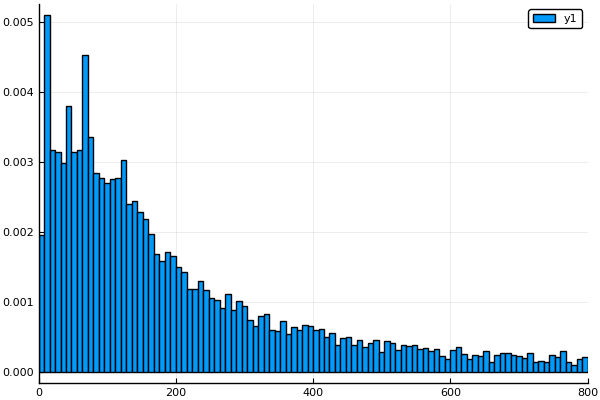
\includegraphics[width=.9\linewidth]{histPDF_Gamma.png}
\end{center}

\section{c}
\label{sec:org6ba1c64}
\begin{minted}[frame=lines,fontsize=\scriptsize,xleftmargin=\parindent,linenos,mathescape,breaklines=true,stripnl=true,firstnumber=last]{julia}

# $\text{(GG):}\quad f(x;\alpha,\beta,m) = \frac{m}{\beta^\alpha \Gamma\left(\frac{\alpha}{m}\right)}x^{\alpha-1}e^{-\left(\frac{x}{\beta}\right)^m},\quad x\in[0,\infty), \:\alpha,\beta,m>0$
function GGammaPDF( α::Float64, β::Float64, m::Float64, x::Float64)
    return ( (m / β^α) * x^(α-1) * exp( - (x / β)^m) ) / gamma( α / m)
end


function GGammaLikelihood( x::Vector{Float64}, α::Real, β::Real, m::Real)
    return log(m) - α*log(β) + (α - 1)*mean(log.(x)) - mean( (x ./ β).^m  ) - lgamma( α / m )    
end

function EstimateGG( data::Vector{Float64}, guess::Vector{Float64})
    #To hard enforce that all of our parameters are positive, we
    #exponentiate them. Limit them to .1 as the lower bound for
    #numerics sake
    θ = log.(guess .- .1)
    fun(x::Vector) = -GGammaLikelihood( data, (exp.(x).+ .1)... )



    result = optimize(fun, θ, Newton(), autodiff=:forward)
end


sln = EstimateGG( healthCosts, [Gamma_̂α, Gamma_̂β, 1.0])

GG_̂α = exp(sln.minimizer[1]) + .1
GG_̂β = exp(sln.minimizer[2]) + .1
GG_̂m = exp(sln.minimizer[3]) + .1
GG_LogLikelihood = -sln.minimum

println( "GG ̂α = ", GG_̂α)
println( "GG ̂β = ", GG_̂β )
println( "GG ̂m = ", GG_̂m )
println( "Likelihood Value: ", GG_LogLikelihood )

result = [["GG \$\\est{\\alpha}\$: ", "GG \$\\est{\\beta}\$: ", "GG \$\\est{m}\$: ","GG Likelihood: " ] cln.([ GG_̂α,  GG_̂β,  GG_̂m, GG_LogLikelihood])]

\end{minted}

\begin{center}
\begin{tabular}{lr}
GG \(\est{\alpha}\): & 1.7396\\
GG \(\est{\beta}\): & 0.1\\
GG \(\est{m}\): & 0.24872\\
GG Likelihood: & -7.0746\\
\end{tabular}
\end{center}

\begin{minted}[frame=lines,fontsize=\scriptsize,xleftmargin=\parindent,linenos,mathescape,breaklines=true,stripnl=true,firstnumber=last]{julia}
histogram( healthClaims[:A], bins=0:8:800, normalize=true, xlims=(0,800),label="Health Claims \$\\leq 800\$")
pdfXVal = range(0.0, 800.0)
#pdfXVal = linspace( minimum(truncatedHealthClaims), maximum(truncatedHealthClaims))
pdfYVal = [GGammaPDF( GG_̂α, GG_̂β, GG_̂m, x ) for x in pdfXVal]


plot!( pdfXVal, pdfYVal, label="Generalized Gamma Estimate" )
savefig( "histPDF_GG.png" )
\end{minted}

\begin{center}
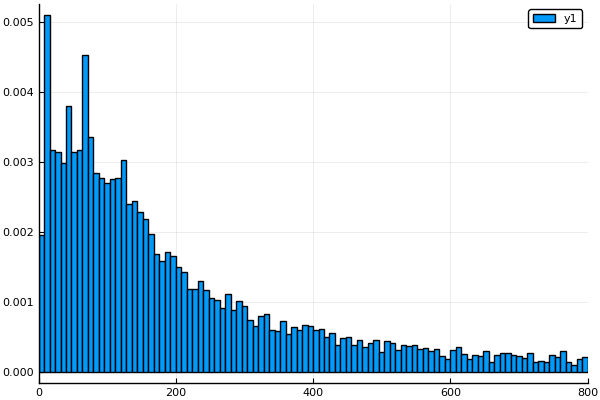
\includegraphics[width=.9\linewidth]{histPDF_GG.png}
\end{center}


\subsection{d}
\label{sec:org83e81e7}
\begin{minted}[frame=lines,fontsize=\scriptsize,xleftmargin=\parindent,linenos,mathescape,breaklines=true,stripnl=true,firstnumber=last]{julia}
function GBetaTwoPDF( x::Float64, a::Real, b::Real, p::Real, q::Real)
    #We require all parameters to be positive, so abs(a) = a
    return a*x^(a*p -1) / (b^(a*p) *beta(p,q)*(1+(x/b)^a)^(p+q))
end



function GBetaTwoLikelihood( x::Vector{Float64}, a::Real, b::Real, p::Real, q::Real)
    return log( a) + (a*p -1)*mean(log.(x)) - (a*p)*log(b) - log(beta(p,q)) - (p+q)*mean( log.( 1 .+(x ./ b).^a ))
end

function EstimateGBetaTwo( data::Vector{Float64}, guess::Vector{Float64})
      #To hard enforce that all of our parameters are positive, we
      #exponentiate them
    θ = log.(guess .- .1)
    #θ = guess
    fun(x::Vector) = -GBetaTwoLikelihood( data, (exp.(x) .+ .1)... )


    #This guy is being fickle, Newton() struggles a little bit, but
    #NewtonTrust seems to outperform LBFGS
    result = optimize(fun, θ, NewtonTrustRegion(), autodiff=:forward, Optim.Options(iterations=2000) )
end

#$GG(\alpha,\beta,m) = \lim_{q\rightarrow\infty}GB2\left(a=m,b=q^{1/m}\beta,p=\frac{\alpha}{m},q\right)$
sln = EstimateGBetaTwo( healthCosts, [GG_̂m, 10000^(1 / GG_̂m) * GG_̂β, GG_̂α / GG_̂m, 10000])

GB2_̂α = exp( sln.minimizer[1]) + .1
GB2_̂β = exp( sln.minimizer[2]) + .1
GB2_̂p = exp( sln.minimizer[3]) + .1
GB2_̂q = exp( sln.minimizer[4]) + .1
GB2_LogLikelihood = -sln.minimum

result = [["GB2 \$\\est{\\alpha}\$: ", "GB2 \$\\est{\\beta}\$: ", "GB2 \$\\est{p}\$: ","GB2 \$\\est{q}\$: ","GB2 Likelihood: " ] cln.([GB2_̂α, GB2_̂β,  GB2_̂p,  GB2_̂q, -sln.minimum])]
\end{minted}

\begin{center}
\begin{tabular}{lr}
GB2 \(\est{\alpha}\): & 1.2714\\
GB2 \(\est{\beta}\): & 143.23\\
GB2 \(\est{p}\): & 1.0299\\
GB2 \(\est{q}\): & 0.84852\\
GB2 Likelihood: & -7.0354\\
\end{tabular}
\end{center}

\begin{minted}[frame=lines,fontsize=\scriptsize,xleftmargin=\parindent,linenos,mathescape,breaklines=true,stripnl=true,firstnumber=last]{julia}
histogram( healthClaims[:A], bins=0:8:800, normalize=true, xlims=(0,800),label="Health Claims \$\\leq 800\$")
pdfXVal = range( 0.0, 800.0)
#pdfXVal = linspace( minimum(truncatedHealthClaims), maximum(truncatedHealthClaims))
pdfYVal = [GBetaTwoPDF( x, GB2_̂α, GB2_̂β, GB2_̂p, GB2_̂q ) for x in pdfXVal]


plot!( pdfXVal, pdfYVal, label="Generalized Beta 2 Estimate" )
savefig( "histPDF_GB2.png" )
\end{minted}

\begin{center}
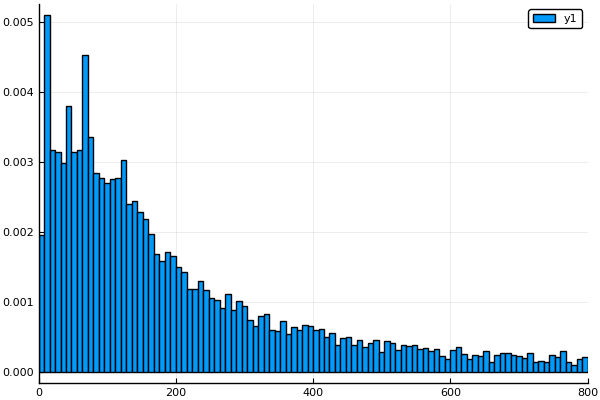
\includegraphics[width=.9\linewidth]{histPDF_GB2.png}
\end{center}

\subsection{e}
\label{sec:org37d2ff9}
Since the likelihood function values at the optimum for parts (b) and
(c) are the constrained maximum likelihood estimators, the likelihood
ratio test is simply: 
\begin{equation*}
  2 \left( f( \est{\theta} - \altest{\theta}) \right) \sim \chi_{p}^{2}
\end{equation*}

Where \(p\) is the number of constraints in the estimation procedure. 
\begin{minted}[frame=lines,fontsize=\scriptsize,xleftmargin=\parindent,linenos,mathescape,breaklines=true,stripnl=true,firstnumber=last]{julia}

# Gamma Has Two restrictions
tStatGamma = 2*(GB2_LogLikelihood - likelihood)
# Generalized Gamma Has One Restriction
tStatGG = 2*(GB2_LogLikelihood - GG_LogLikelihood)

results = [["", "Gamma", "Generalized Gamma"] [ "\$\\chi^{2}\$", cln(tStatGamma), cln(tStatGG)] ["p-value",  cln(1.0 - cdf(Chisq(4),tStatGamma)), cln(1.0 - cdf( Chisq(4),tStatGG)) ] ]
\end{minted}

\begin{center}
\begin{tabular}{lrr}
 & \(\chi^{2}\) & p-value\\
Gamma & 0.56771 & 0.96658\\
Generalized Gamma & 0.078294 & 0.99925\\
\end{tabular}
\end{center}

\subsection{f}
\label{sec:org638d3ea}
The Probability that someone has a health care claim of more than
\$$\backslash$\(1000\) is given by:

\begin{align*}
  \Pr( X > 1000) &= 1 - \Pr( X \leq 1000)\\
                 &= \int_0^{1000}f_Xdx
\end{align*}

However, since the integral of a Generalized Beta 2 Distribution is
quite nasty, I shall compute it numerically.

\begin{minted}[frame=lines,fontsize=\scriptsize,xleftmargin=\parindent,linenos,mathescape,breaklines=true,stripnl=true,firstnumber=last]{julia}
f(x) = GBetaTwoPDF( x, GB2_̂α, GB2_̂β, GB2_̂p, GB2_̂q )
area = quadgk( f, 0, 1000 )[1]
output = ["Probability of Having > 1000: " cln(1-area)]
\end{minted}

\begin{center}
\begin{tabular}{lr}
Probability of Having > 1000: & 0.11766\\
\end{tabular}
\end{center}



\section{Question 2}
\label{sec:org36206b2}

\subsection{a}
\label{sec:org3a3570a}

Equations (3) and (5) tell us that


\begin{align*}
  w_t - (1-\alpha) exp( z_t ) (k_t)^{\alpha-1} &= 0\\
  z_t = \rho z_{t-1} + (1-\rho)\mu &+ \epsilon_t
\end{align*}

Taking logs of equation (3):
\begin{align*}
  \log w_t &= \log ( 1- \alpha) + z_t + (\alpha-1) \log k_t\\
  z_t &= \log w_t - \log ( 1- \alpha) - (\alpha-1) \log k_t
\end{align*}

This tells us that for $t > 1$
\begin{align*}
  \log w_t - \log ( 1- \alpha) - (\alpha-1) \log k_t &\sim \normal\left( \rho z_{t-1} +
                                             (1-\rho)\mu, \sigma^2 \right)\\
  &\sim \normal\left( \rho\left( \log w_{t-1} - \log( 1- \alpha) -(\alpha-1) \log
    k_{t-1} \right) + (1-\rho)\mu, \sigma^2 \right)
\end{align*}

For $t=1$
\begin{equation*}
  \log w_1 - \log ( 1- \alpha) - (\alpha-1) \log k_1 \sim \normal( \mu, \sigma^2)
\end{equation*}


We may now estimate this model using Maximum Likelihood Estimation

\begin{minted}[frame=lines,fontsize=\scriptsize,xleftmargin=\parindent,linenos,mathescape,breaklines=true,stripnl=true,firstnumber=last]{julia}
#$\normal\left( \rho\left( \log w_{t-1} - \log( 1- \alpha) -(\alpha-1) \log k_{t-1} \right) + (1-\rho)\mu, \sigma^2 \right)$

#Clean it up when it exists, comes in the order: (c, k, w, r)
macroData = DataFrame(load("MacroSeries.csv", header_exists=false, colnames=["C", "K", "W", "R"]))

w = convert( Vector{Float64}, macroData[:W] )
k = convert( Vector{Float64}, macroData[:K] )

function LogLikelihood( N, w::Vector{Float64}, k::Vector{Float64}, α::Real, ρ::Real, μ::Real, σ²::Real  )
    #The pdf of a normal: $\frac{1}{\sqrt{2 \pi \sigma^2}} \exp( - \frac{ (x-\mu)^2}{2 \sigma^2})$
    #Log Likelihood: $- \frac{1}{2} \log \sigma^2 - \frac{ (x-\mu)^2}{ 2 \sigma^2}$

    logLik = -.5*log(σ²)- ( log(w[1]) - log(1-α) - (1-α)*log(k[1]) - μ)^2 / (2*σ²)

    #Note we do not have the -.5*log(2*pi)
    #Because that does not matter at all for MLE estimation.
    for i in 2:N
        mean = ρ*(log(w[i-1]) - log( 1 - α)  - (α-1)*log( k[i-1])) + (1-ρ)*μ
        logLik += -.5*log( σ² ) - (  (log(w[i]) - log(1-α) - (1-α)*log(k[i]) - mean)^2 / (2*σ²))
    end
    return logLik
end

N = length(w)

α₀ = .5
β = .99
μ₀ = 1.0
σ₀ = 1.0
ρ₀ = 0.0

#We parameterize each of the variables so that they meet their constraints.
# tanh is used to ensure that $\rho \in (-1,1)$
θ = zeros(4)
θ[1] = log( α₀ / ( 1 - α₀) )
θ[2] = atanh( ρ₀)
θ[3] = log( μ₀ )
θ[4] = log( σ₀)


fun(x::Vector) = -LogLikelihood( N, w, k, exp(x[1]) / (1 + exp(x[1])), tanh(x[2]), exp(x[3]), exp(x[4])  )

result = optimize(fun, θ, Newton(), autodiff=:forward)

model_̂θ = result.minimizer

model_̂α = exp(model_̂θ[1]) / (1 + exp(model_̂θ[1]))
model_̂ρ = tanh(model_̂θ[2])
model_̂μ = exp(model_̂θ[3])
model_̂σ = exp(model_̂θ[4])

output = [["\$\\est{\\alpha}\$:", "\$\\est{\\rho}\$:", "\$\\est{\\mu}\$:", "\$\\est{\\sigma^{2}}\$:"]  cln.([model_̂α, model_̂ρ, model_̂μ, model_̂σ])]
\end{minted}

\begin{center}
\begin{tabular}{lr}
\(\est{\alpha}\): & 0.1128\\
\(\est{\rho}\): & 0.0013758\\
\(\est{\mu}\): & 2.1987\\
\(\est{\sigma^{2}}\): & 0.0095002\\
\end{tabular}
\end{center}

\begin{minted}[frame=lines,fontsize=\scriptsize,xleftmargin=\parindent,linenos,mathescape,breaklines=true,stripnl=true,firstnumber=last]{julia}
#Sadly Optim.jl does not automatically report the hessian, though I am
 #sure it is obtainable. So we will use forward-mode automatic
 #differentiation to obtain this hessian. However it does not always
 #return symmetric matrices, so we will make the matrix symmetric then
 #invert it using the cholesky decomposition to be numerically stable.
 hess = ForwardDiff.hessian(fun, result.minimizer)
 for i in 1:4
     for j in 1:i
         if i == j
             continue
         end
         hess[i,j] = (hess[i,j]+hess[j,i])*.5
         hess[j,i] = hess[i,j]
     end
 end
 F = cholesky(hess)
 #F.L * F.U = H
 hessInv = cln.(F.U \ (F.L \ I))
\end{minted}

\begin{center}
\begin{tabular}{rlrl}
0.22705 & 0.00017156 & 0.17324 & -5.1778 \texttimes{} 10\(^{\text{-16}}\)\\
0.00017156 & 1.2065 \texttimes{} 10\(^{\text{-05}}\) & -2.018 \texttimes{} 10\(^{\text{-05}}\) & 4.6392 \texttimes{} 10\(^{\text{-18}}\)\\
0.17324 & -2.018 \texttimes{} 10\(^{\text{-05}}\) & 0.13412 & -4.5417 \texttimes{} 10\(^{\text{-16}}\)\\
-5.1778 \texttimes{} 10\(^{\text{-16}}\) & 4.6392 \texttimes{} 10\(^{\text{-18}}\) & -4.5417 \texttimes{} 10\(^{\text{-16}}\) & 0.02\\
\end{tabular}
\end{center}

\section{b}
\label{sec:orga026be5}

Equations (4) and (5) read:
\begin{align*}
  r_t - \alpha \exp( z_t ) k_t^{\alpha -1 } &= 0\\
  z_t = \rho z_{t-1} + (1-\rho)\mu &+ \epsilon_t\\
  \epsilon_t \sim \normal( 0, \sigma^2)
\end{align*}

Taking logs and isolating $z_t$
\begin{align*}
  \log r_t  &= \log \alpha + (\alpha-1) \log k_t + z_t\\
  z_t &= \log \alpha + (\alpha-1) \log k_t - \log r_t
\end{align*}

For $t > 1$:
\begin{align*}
  \log \alpha + (\alpha-1) \log k_t - \log r_t &\sim \normal\left( \rho z_{t-1} +
                                       (1-\rho)\mu, \sigma^2 \right)\\
  &\sim \normal\left( \rho\left( \log \alpha + (\alpha-1)\log k_{t-1} - \log r_{t-1}
    \right) + (1-\rho)\mu, \sigma^2 \right)
\end{align*}

For $t = 1$:
\begin{equation*}
  \log \alpha + (\alpha-1)\log k_1 - \log r_1 \sim \normal( \mu, \sigma^2)
\end{equation*}

This can be estimated using an MLE.

\begin{minted}[frame=lines,fontsize=\scriptsize,xleftmargin=\parindent,linenos,mathescape,breaklines=true,stripnl=true,firstnumber=last]{julia}

r = convert( Vector{Float64}, macroData[:R] )
k = convert( Vector{Float64}, macroData[:K] )

#$\log r_t - \log \alpha - z_t - (\alpha - 1 ) \log k_t = 0$

function LogLikelihood( N, w::Vector{Float64}, k::Vector{Float64}, α::Real, ρ::Real, μ::Real, σ²::Real  )
    #The pdf of a normal: $\frac{1}{\sqrt{2 \pi \sigma^2}} \exp( - \frac{ (x-\mu)^2}{2 \sigma^2})$
    #Log Likelihood: $- \frac{1}{2} \log \sigma^2 - \frac{ (x-\mu)^2}{ 2 \sigma^2}$

    logLik = -.5*log(σ²) - (log(α) + (α-1)*log(k[1]) - log(r[1]) - μ)^2 / (2*σ² )
    #Note the way that the model is structured is: F(...) = 0, so we
    #are maximizing the likelihood of getting a 0 returned for all the
    #moments

    for i in 2:N
        mean = ρ*(log(α) + (α-1)*log(k[i-1]) - log(r[i-1])) + (1-ρ)*μ
        logLik += -.5*log( σ² ) - (  (log(α) + (α-1)*log(k[i]) - log(r[i]) - mean)^2 / (2*σ²))
    end
    return logLik
end

N = length(w)

# α₀ = .5
# β = .99
# μ₀ = 1.0
# σ₀ = 1.0
# ρ₀ = .99
  α₀ = .5
  β = .99
  μ₀ = 1.0
  σ₀ = 1.0
  ρ₀ = 0.0

# #We param
eterize each of the variables so that they meet their constraints.
# tanh is used to ensure that $\rho \in (-1,1)$
θ = zeros(4)
θ[1] = log( α₀ / ( 1 - α₀) )
θ[2] = atanh( ρ₀)
θ[3] = log( μ₀ )
θ[4] = log( σ₀)

#This clamp on the logistic function is quite the hack, since this
#function shouldn't get to 0 or 1, but it was getting stuck at 1
fun(x::Vector) = -LogLikelihood( N, w, k, (exp(x[1]) / (1 + exp(x[1])))*.9+.05, tanh(x[2]), exp(x[3]), exp(x[4])  )

result = optimize(fun, θ, Newton(), autodiff=:forward)

model_̂θ = result.minimizer

model_̂α = (exp(model_̂θ[1]) / (1 + exp(model_̂θ[1])))*.9+.05
model_̂ρ = tanh(model_̂θ[2])
model_̂μ = exp(model_̂θ[3])
model_̂σ = exp(model_̂θ[4])

output = [["\$\\est{\\alpha}\$:", "\$\\est{\\rho}\$:", "\$\\est{\\mu}\$:", "\$\\est{\\sigma^{2}}\$:"]  cln.([model_̂α, model_̂ρ, model_̂μ, model_̂σ])]
\end{minted}

\begin{center}
\begin{tabular}{lr}
\(\est{\alpha}\): & 0.95\\
\(\est{\rho}\): & 0.99102\\
\(\est{\mu}\): & 8.2563 \texttimes{} 10\(^{\text{-15}}\)\\
\(\est{\sigma^{2}}\): & 0.02061\\
\end{tabular}
\end{center}

\begin{minted}[frame=lines,fontsize=\scriptsize,xleftmargin=\parindent,linenos,mathescape,breaklines=true,stripnl=true,firstnumber=last]{julia}

#Sadly Optim.jl does not automatically report the hessian, though I am
 #sure it is obtainable. So we will use forward-mode automatic
 #differentiation to obtain this hessian. However it does not always
 #return symmetric matrices, so we will make the matrix symmetric then
 #invert it using the cholesky decomposition to be numerically stable.
 hess = ForwardDiff.hessian(fun, result.minimizer)
 for i in 1:4
     for j in 1:i
         if i == j
             continue
         end
         hess[i,j] = (hess[i,j]+hess[j,i])*.5
         hess[j,i] = hess[i,j]
     end
 end
 F = cholesky(hess)
 #F.L * F.U = H
 hessInv = cln.(F.U \ (F.L \ I))
\end{minted}

\begin{center}
\begin{tabular}{rrrr}
2.2698 \texttimes{} 10\(^{\text{12}}\) & -0.023973 & 0.0088919 & -0.014286\\
-0.023973 & 0.88359 & 0.031051 & 3.9818 \texttimes{} 10\(^{\text{-16}}\)\\
0.0088919 & 0.031051 & 3.0942 \texttimes{} 10\(^{\text{12}}\) & 0.02\\
-0.014286 & 3.9818 \texttimes{} 10\(^{\text{-16}}\) & 0.02 & 0.02\\
\end{tabular}
\end{center}

\subsection{c}
\label{sec:orga31d249}
From the derivation of the distribution of $\log r_t$ in part (b):

\begin{align*}
    \Pr( r_t > 1) &= \Pr( \log r_t > 0)\\
                  &= \Pr( \log \alpha + z_t + (\alpha - 1)\log k_t > 0)\\
                  &= \Pr( \log \alpha + \rho z_{t-1} + (1 - \rho)\mu + \epsilon_t + (\alpha-1) \log k_t > 0)\\
    &= \Pr( \log(\alpha) + \rho z_{t-1} + (1-\rho)\mu + \frac{Z}{\sigma} + (\alpha-1) \log k_t
      > 0)\\
                  &= \Pr( Z > - \sigma ( \log(\alpha) + \rho z_{t-1} + (1-\rho)\mu + (\alpha-1)\log k_t))\\
    &= 1 - \Pr( Z \leq - \sigma ( \log(\alpha) + \rho z_{t-1} + (1-\rho)\mu + (\alpha-1)\log
      k_t))\\
                  &= \Phi( - \sigma ( \log(\alpha) + \rho z_{t-1} + (1-\rho)\mu + (\alpha-1)\log k_t ))\\
    &\approx \Phi( -\est{\sigma} ( \log \est{\alpha} + \est{\rho}10 + (1-\est{\rho})
      \est{\mu} + (\est{\alpha} - 1) \log( 7,500,000) ))\\
  \end{align*}

\begin{minted}[frame=lines,fontsize=\scriptsize,xleftmargin=\parindent,linenos,mathescape,breaklines=true,stripnl=true,firstnumber=last]{julia}
  prob = cdf( Normal(), -sqrt(model_̂σ)*( log(model_̂α) + model_̂ρ*10 + (1-model_̂ρ)*model_̂μ + (model_̂α-1)*log( 7500000)))
result = ["Prob" cln(prob)]

\end{minted}

\begin{center}
\begin{tabular}{lr}
Prob & 0.2541\\
\end{tabular}
\end{center}
\end{document}